\documentclass{elbioimp2}
\usepackage[utf8]{inputenc}

\usepackage[backend=biber,style=vancouver]{biblatex}
\usepackage{csquotes}
  
\title{This is your template for Journal of Electrical Bioimpedance}
\shorttitle{Short version of title}
\author{First B. Author\affiliation{Department, University, City,
    Country}, Second C. Coauthor\affiliation{Company, City,
    Country} and Last Author\affiliation{E-mail any correspondence to:
  myname@domain.com}} 
\shortauthor{Author et al.}
\elbioimpreceived{1 Jan 2019}  
\elbioimppublished{21 Jul 2019}
\elbioimpfirstpage{11}
\elbioimpvolume{10}
\elbioimpyear{2020}
 
\addbibresource{demo.bib}

\begin{document}
\maketitle

\begin{abstract}
  These are guidelines for preparing papers for the \emph{Journal of
  Electrical Bioimpedance}. The journal accepts original research
  papers and review articles within the broad field of electrical
  bioimpedance. Use this document as a template if you are using
  \LaTeX; otherwise, use this document as an
  instruction set. The paper size is A4 (21 × 29.7\,cm).  

  \keywords{Bioimpedance; current; voltage}
\end{abstract}

\section{Introduction}
This document is a template for \LaTeX. 
Please use the electronic version of this document as a
template when you produce your manuscript for submission to the
\emph{Journal of Electrical Bioimpedance}. The paper size is A4 (21 × 
29.7~cm).

The introduction section of your paper should include the necessary
background information, including an adequate review of earlier
findings and the justification for conducting this study.

\section{Materials and methods}
The margins in this document are set to 2.5\,cm for the top and 1.5\,cm
for the sides and bottom. The main body of the manuscript is in two
columns separated by a 1\,cm. The line spacing is 1.1, and the
references list has 3\,pt spacing between each reference.

Body text is \emph{Computer Modern Bright} (which is quite similar to
Calibri) at 10\,pt. Level~1 headings are in bold and level~2
headings are in italic.

In the materials and methods section, please describe all necessary
details on how the study was performed. Do not
include any discussions of the work in this section. Enough
information should be given so that other researchers can reproduce
your study.

\subsection{Informed consent}
Informed consent has been obtained from all individuals included in
this study. (Keep this sentence if applicable.)

\subsection{Ethical approval}
The research related to human use has been complied with all relevant
national regulations, institutional policies and in accordance with
the tenets of the Helsinki Declaration, and has been approved by the
authors’ institutional review board or equivalent committee.

The research related to animals use has been complied with all the
relevant national regulations and institutional policies for the care
and use of animals.

The conducted research is not related to either human or animal use.

(Keep one of these sentences as applicable.)

\section{Results}
All figures should be numbered consecutively with the figure legend
indented 0.5\,cm on each side. See figure~\ref{box-plot} for an example.
Figures may be in color or black and white and must be of such quality
that they produce clear and sharp printouts on an ordinary (color)
laser printer.

\subsection{What to include}
Use this section to present the results from the measurements or
studies that were described in the last section, but without going
into any discussion about the results.

\begin{figure}[htp]
  \centering
  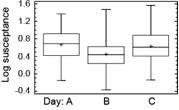
\includegraphics[width=0.7\columnwidth]{test-ill}
  \caption{Box-plot showing median value (line), mean value (cross),
    middle 50\,\% (box) and smallest and largest point within 
    1.5~interquartiles from the box (whiskers) of all measurements
    on days A, B and~C.\label{box-plot}}
\end{figure}

\section{Discussion}
Now you can discuss your results. Emphasize the new and important
aspects of the study and the conclusions that follow from them. Do not
repeat in detail data or other information given in the Introduction
or the Results section. After this section there may be sections
called Conclusion and Acknowledgments. The last section is References.

\subsection{Reference style}
The \emph{Journal of Electrical Bioimpedance} uses primarily the Vancouver
style of references with numbers in square brackets in the text and a
numbered list in the Reference section.\cite{biomed-req} However, using the
Harvard reference style will also be accepted in some cases.

\subsection{Conflict of interest}
Authors state no conflict of interest. (Either keep this sentence or
describe any comflict of interest.)

\newpage
\nocite{*}
\printbibliography
\end{document}
